\documentclass{article}
\usepackage{graphicx,amsmath,latexsym}
\usepackage{color,psfrag,boxedminipage,amssymb}
\usepackage{tikz}
\usepackage{pgf}
\usepackage{extarrows}
\usepackage{amssymb}
\usepackage{amsmath}


\usetikzlibrary{positioning,arrows}

\newcommand{\st}{\ensuremath{\boldsymbol{s}_k(\boldsymbol{\theta})}}
\newcommand{\St}{{\mathbf S}\ensuremath{(\boldsymbol{\theta})}}
\newcommand{\phibf}{\ensuremath{\boldsymbol{\phi}}}
\newcommand{\varphibf}{\ensuremath{\boldsymbol{\varphi}}}
\def \phibfh{\ensuremath{\hat{\boldsymbol{\phi}}}}
\renewcommand{\sp}{\ensuremath{\boldsymbol{s}(\boldsymbol{\phi})}}
\newcommand{\hp}{\ensuremath{\boldsymbol{h}(\boldsymbol{\phi})}}
\newcommand{\thk}{\ensuremath{\boldsymbol{\theta}_k}}
\renewcommand{\th}{\ensuremath{\boldsymbol{\theta}}}
\newcommand{\alp}{\ensuremath{\boldsymbol{\alpha}}}
\def \thh{\ensuremath{\hat{\boldsymbol{\theta}}}}
\def \epsbf{\ensuremath{\boldsymbol{\epsilon}}}
\def \tht{\tilde{\th}}
\newcommand{\mubf}{\ensuremath{\boldsymbol{\mu}}}

\newcommand{\ctft}{\buildrel{{\cal F}}\over{\longleftrightarrow}}
\newcommand{\defin}{\buildrel{\triangle}\over{=}}

\def \Em{{\mathbb{E}}}


\def \abf{{\mathbf a}}
\def \Abf{{\mathbf A}}
\def \bbf{{\mathbf b}}
\def \Bbf{{\mathbf B}}
\def \cbf{{\mathbf C}}
\def \Cbf{{\mathbf C}}
\def \dbf{{\mathbf d}}
\def \Dbf{{\mathbf D}}
\def \ebf{{\mathbf e}}
\def \Ebf{{\mathbf E}}
\def \fbf{{\mathbf f}}
\def \Fbf{{\mathbf F}}
\def \gbf{{\mathbf g}}
\def \Gbf{{\mathbf G}}
\def \hbf{{\mathbf h}}
\def \Hbf{{\mathbf H}}
\def \ibf{{\mathbf i}}
\def \Ibf{{\mathbf I}}
\def \jbf{{\mathbf j}}
\def \Jbf{{\mathbf J}}
\def \kbf{{\mathbf k}}
\def \Kbf{{\mathbf K}}
\def \lbf{{\mathbf l}}
\def \Lbf{{\mathbf L}}
\def \mbf{{\mathbf m}}
\def \Mbf{{\mathbf M}}
\def \nbf{{\mathbf n}}
\def \Nbf{{\mathbf N}}
\def \obf{{\mathbf o}}
\def \Obf{{\mathbf O}}
\def \pbf{{\mathbf p}}
\def \Pbf{{\mathbf P}}
\def \qbf{{\mathbf q}}
\def \Qbf{{\mathbf Q}}
\def \rbf{{\mathbf r}}
\def \Rbf{{\mathbf R}}
\def \sbf{{\mathbf s}}
\def \Sbf{{\mathbf S}}
\def \tbf{{\mathbf t}}
\def \Tbf{{\mathbf T}}
\def \ubf{{\mathbf u}}
\def \Ubf{{\mathbf U}}
\def \vbf{{\mathbf v}}
\def \Vbf{{\mathbf V}}
\def \wbf{{\mathbf w}}
\def \Wbf{{\mathbf W}}
\def \xbf{{\mathbf x}}
\def \Xbf{{\mathbf X}}
\def \ybf{{\mathbf y}}
\def \Ybf{{\mathbf Y}}
\def \zbf{{\mathbf z}}
\def \Zbf{{\mathbf Z}}
\def \0bf{{\mathbf 0}}

\def \Emean{\mathbb{E}}

\def \Sibf{{\mathbf \Sigma}}
\def \xbbf{\mathbf{\bar{x}}}
\def \etr{\mbox{etr}}
\def \tr{\mbox{tr}}
\def \Tr{\mbox{Tr}}
\def \Cov{\mbox{Cov}}
\def \cost{\mbox{cost}}
\def \diag{\mbox{diag}}
\def \Lambf{{\mathbf{\Lambda}}}
\def \Gambf{{\mathbf{\Gamma}}}
\def \Sigbf{{\mathbf \Sigma}}
\newcommand{\rhobf}{\ensuremath{\boldsymbol{\rho}}}
\newcommand{\lambf}{\ensuremath{\boldsymbol{\lambda}}}
\newcommand{\nubf}{\ensuremath{\boldsymbol{\nu}}}

\newcounter{examplenr}[section]
\renewcommand{\theexamplenr}{\arabic{examplenr}}%{\thesection.\arabic{examplenr}}
\newenvironment{example}[1]{\vskip \baselineskip
\refstepcounter{examplenr}\noindent{{\bf
Example~\theexamplenr}\hskip .5em #1\\} }{\hrulefill $\Box$
 \vskip\baselineskip}



\newcounter{theoremnr}[section]
%\renewcommand{\thetheoremnr}{\thesection.\arabic{theoremnr}}
\renewcommand{\thetheoremnr}{\arabic{theoremnr}}
\newtheorem{A}[theoremnr]{Theorem}
\newcounter{theoremProofnr}[section]
%\renewcommand{\thetheoremProofnr}{\thesection.\arabic{theoremProofnr}}
\renewcommand{\thetheoremProofnr}{\arabic{theoremProofnr}}
\newtheorem{B}[theoremProofnr]{Proof of Theorem}
\newcounter{corollarynr}[section]
\renewcommand{\thecorollarynr}{\thesection.\arabic{corollarynr}}
\newtheorem{C}[corollarynr]{Corollary}
\newcounter{Lemmanr}[section]
\renewcommand{\theLemmanr}{\thesection.\arabic{Lemmanr}}
\newtheorem{D}[Lemmanr]{Lemma}
\newcounter{LemmaProofnr}[section]
\renewcommand{\theLemmaProofnr}{\thesection.\arabic{LemmaProofnr}}
\newtheorem{E}[LemmaProofnr]{Proof of Lemma}

\newcounter{propositionnr}[section]
\renewcommand{\thepropositionnr}{\arabic{propositionnr}}
\newtheorem{F}[propositionnr]{Proposition}
\newcounter{propositionProofnr}[section]
\renewcommand{\thepropositionProofnr}{\arabic{propositionProofnr}}
\newtheorem{G}[propositionProofnr]{Proof of proposition}

\newenvironment{working}{\color{blue}\sffamily\em}{}
\newenvironment{forslag}{\color{red}\sffamily\em}{}

\newcounter{definnr}[section]
\renewcommand{\thedefinnr}{\arabic{definnr}}
\newtheorem{J}[definnr]{Definition}

\newcommand{\norm}[1]{\lVert #1 \rVert}
\renewcommand {\P}[1]{\mathbb{P}[ #1 ]}
\newcommand{\Equiv}{\xLeftrightarrow[]{}}

\newdimen\mytoplen
\newdimen\mybotlen
\def\equiv#1#2{%
	\settowidth\mytoplen{$\scriptstyle\text{#1}$}%
	\settowidth\mybotlen{$\scriptstyle\text{#2}$}%
	\def\mysubparbox##1##2{%
		\text{\parbox{.6##1}{%
				\rightskip=0pt plus 1fill%
				\leftskip=0pt plus 1fill%
				\baselineskip=5pt ##2}}}
\xLeftrightarrow[\mysubparbox{\mybotlen}{#2}]{\mysubparbox{\mytoplen}{#1}}}%

\def\Implies#1#2{%
	\settowidth\mytoplen{$\scriptstyle\text{#1}$}%
	\settowidth\mybotlen{$\scriptstyle\text{#2}$}%
	\def\mysubparbox##1##2{%
		\text{\parbox{.6##1}{%
				\rightskip=0pt plus 1fill%
				\leftskip=0pt plus 1fill%
				\baselineskip=5pt ##2}}}
\xRightarrow[\mysubparbox{\mybotlen}{#2}]{\mysubparbox{\mytoplen}{#1}}}%

\def\equals#1#2{%
	\settowidth\mytoplen{$\scriptstyle\text{#1}$}%
	\settowidth\mybotlen{$\scriptstyle\text{#2}$}%
	\def\mysubparbox##1##2{%
		\text{\parbox{.6##1}{%
				\rightskip=0pt plus 1fill%
				\leftskip=0pt plus 1fill%
				\baselineskip=5pt ##2}}}
	\xlongequal [\mysubparbox{\mybotlen}{#2}]{\mysubparbox{\mytoplen}{#1}}}%

% http://texblog.net/latex-archive/maths/amsmath-matrix/
\makeatletter
\renewcommand*\env@matrix[1][*\c@MaxMatrixCols c]{%
	\hskip -\arraycolsep
	\let\@ifnextchar\new@ifnextchar
	\array{#1}}
\makeatother
%$A \xLeftrightarrow[\substack{theorem\\formula}]{\substack{mean\\value}}B$


\newcommand{\R}{\mathbb{R}}
\newcommand{\Z}{\mathbb{Z}}
\newcommand{\N}{\mathbb{N}}

\def\pd#1#2{\frac{\partial #1}{\partial #2}}

\def\d#1#2{\frac{\delta #1}{\delta #2}}


\newcommand{\equivtext}[1]{\ensuremath{\stackrel{\text{#1}}{\Equiv}}}
\newcommand{\approxtext}[1]{\ensuremath{\stackrel{\text{#1}}{\approx}}}
\newcommand{\equalstext}[1]{\ensuremath{\stackrel{\text{#1}}{=}}}
\newcommand{\impliestext}[1]{\ensuremath{\stackrel{\text{#1}}{\Rightarrow}}}
\usepackage{amsmath}
\usepackage{geometry}
\usepackage{caption}
\usepackage{lipsum} 
\geometry{a4paper}
\usepackage[backend=biber,style=ieee]{biblatex}
\usepackage{comment}
\usepackage{mathtools}
\usepackage{xparse}
\usepackage{pgfmath}
\usepackage{etoolbox}
\usepackage{multicol}
\usepackage{listings}

\usepackage{graphicx}
\usepackage{subfig}
\usepackage{breqn}
\graphicspath{ {img/} }
\setlength{\columnsep}{1cm}

\bibliography{ref.bib}

\begin{document}

\title{\textbf{Large Scale Data Analysis Exam}}
\author{\textbf{Lucian Tirca (hrn947@alumni.ku.dk)}}
\maketitle


\section{Deep Learning}
\subsection{Variance}
\begin{lstlisting}[language={},numbers=left,numberstyle=\tiny,frame = single]
Variance for redshift is 0.010498
\end{lstlisting}

\begin{lstlisting}[language={},numbers=left,numberstyle=\tiny,frame=single,breaklines=true,postbreak=\mbox{\textcolor{red}{$\hookrightarrow$}\space}]
Iteration: 30000 / 30000
final training accuracy: 0.000976738
final test accuracy:  0.00126395 
final validation accuracy:  0.0010332
INFO:tensorflow:Restoring parameters from tensor_logs/bestNetwork
best training accuracy: 0.000954459 
best test accuracy:  0.00125532 
best validation accuracy:  0.000915237
\end{lstlisting}

\subsection{Deep Network for Regression}
I have tested both the GradientdescentOptimizer and the AdamOptimizer, and saw that the AdamOptimizer is superior in performance. However, plots of both are available below.

Some of the lines I have changed were:

\begin{lstlisting}[language=python,numbers=left,numberstyle=\tiny,frame=single,breaklines=true,postbreak=\mbox{\textcolor{red}{$\hookrightarrow$}\space}]
#change the activation to ReLU
y_1 = tf.matmul(x_data , W_1 ) + b_1
y_1 = tf.nn.relu(y_1)
\end{lstlisting}

\begin{lstlisting}[language=python,numbers=left,numberstyle=\tiny,frame=single,breaklines=true,postbreak=\mbox{\textcolor{red}{$\hookrightarrow$}\space}]
#change the loss function to MSE
loss = tf.reduce_mean(tf.square(model_output - y_target), name='mean_squared_error')
\end{lstlisting}

\begin{lstlisting}[language=python,numbers=left,numberstyle=\tiny,frame=single,breaklines=true,postbreak=\mbox{\textcolor{red}{$\hookrightarrow$}\space}]
#change the optimizer to ADAM
# Declare optimizer
my_opt =  tf.train.AdamOptimizer(FLAGS.lr)
train_step = my_opt.minimize(loss)
\end{lstlisting}

\subsection{TensorBoard}

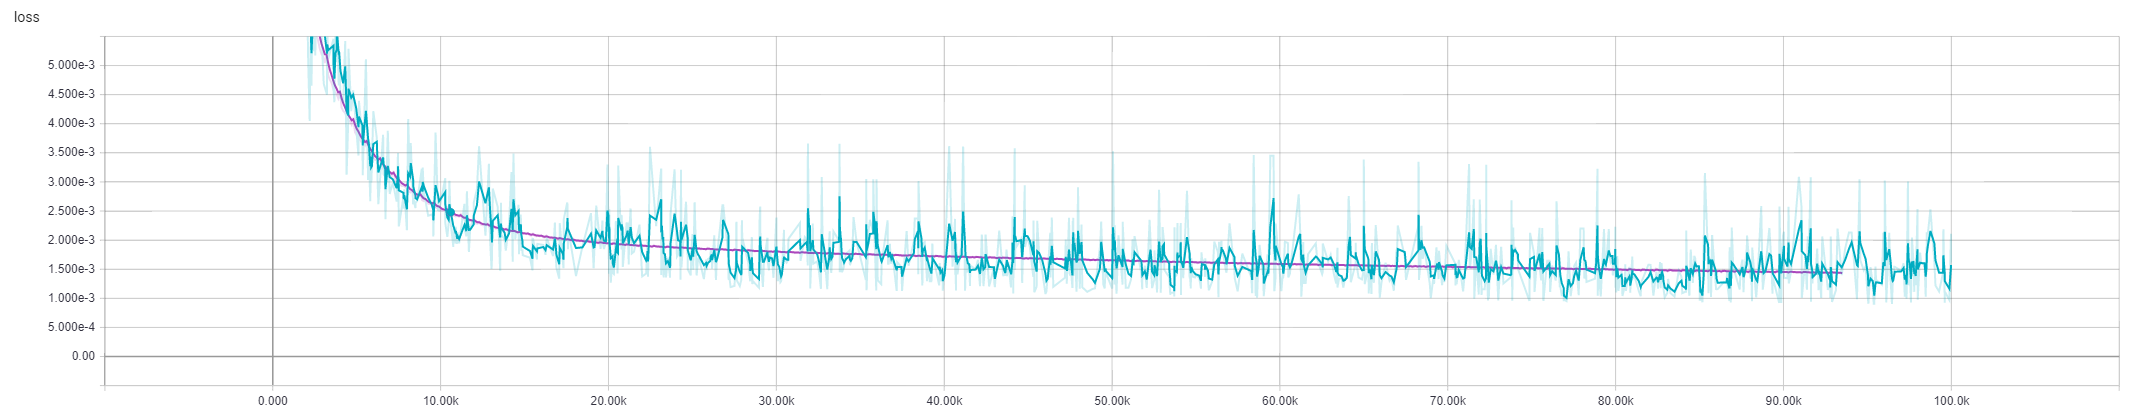
\includegraphics[width=15cm]{tf_relu_gradientdescent.png}

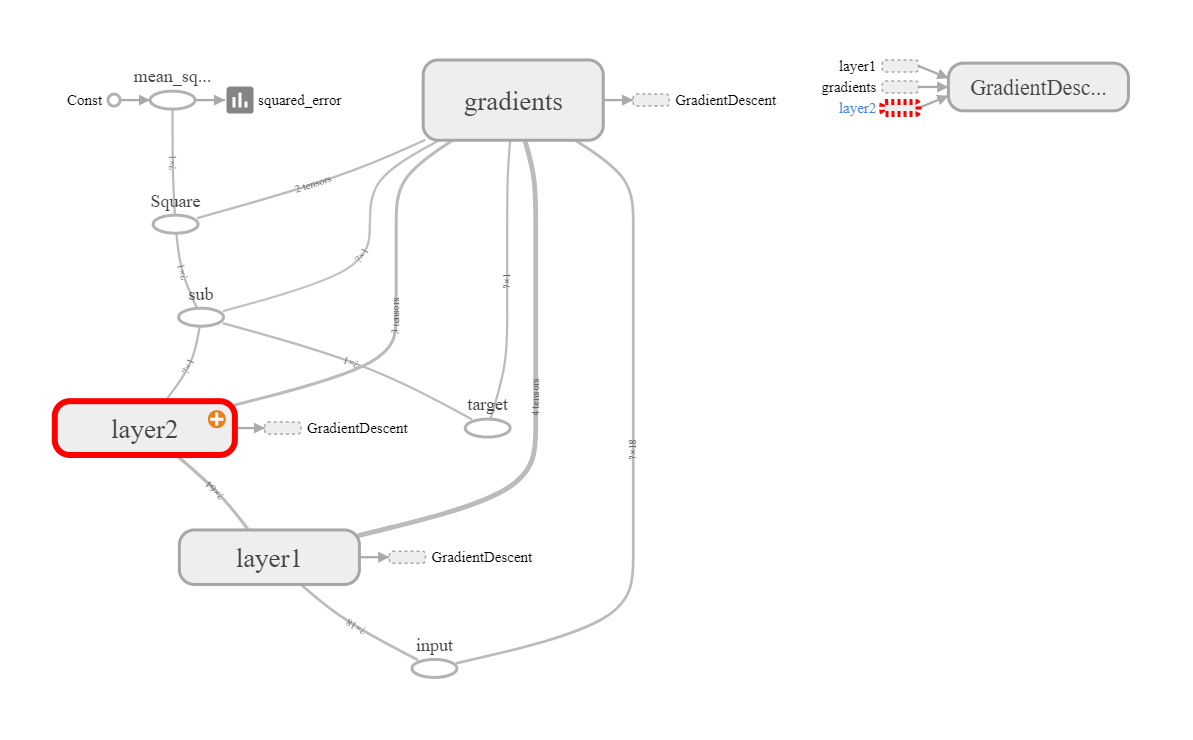
\includegraphics[width=13cm]{graph_relu_gradientdescent.png}

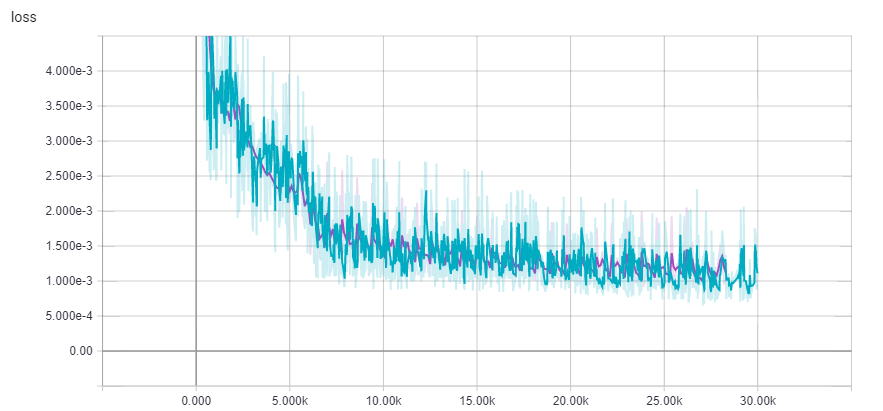
\includegraphics[width=15cm]{tf_relu_adam.png}

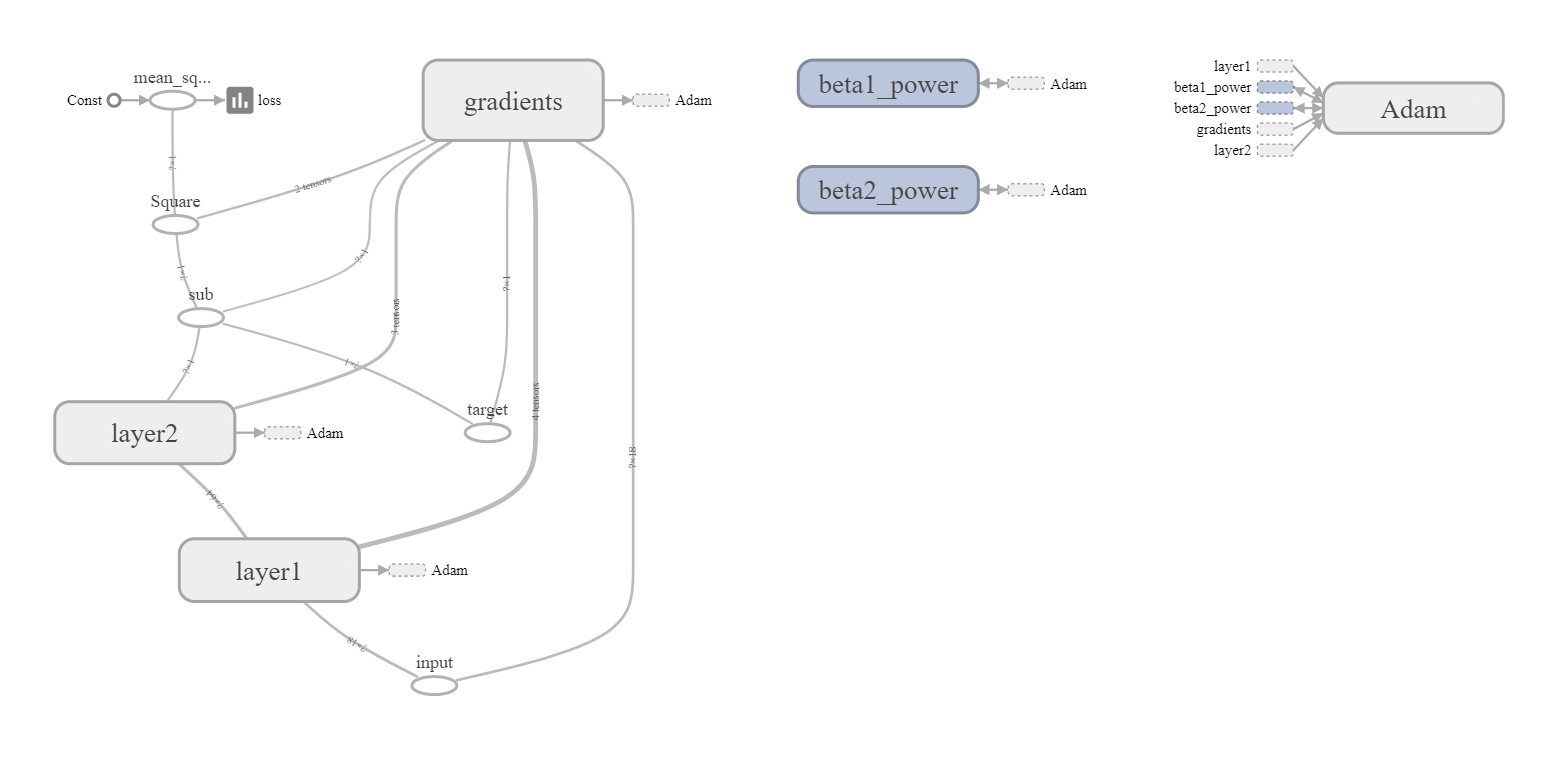
\includegraphics[width=13cm]{graph_relu_adam.png}


\section{Nearest Neighbors}
\begin{lstlisting}[language={},numbers=left,numberstyle=\tiny,frame = single]
Fitting for columns [0, 1, 2, 8, 9] for validation...
CPU times: user 2.44 s, sys: 4 ms, total: 2.45 s
Wall time: 721 ms
Best MSE for Validation is 0.188903 ...
Fitting for columns [0, 1, 2, 8, 9] for test...
CPU times: user 26 s, sys: 64 ms, total: 26.1 s
Wall time: 6.87 s
Best MSE for test is 0.223736 ...
\end{lstlisting}


\section{Locality Sensitive Hashing}
\subsection{Brute Force}
Due to a omission in my code (forgetting to convert the sparse Jaccard similarity matrix to dense after computing the dot product $Q \cdot P^T$), the computation took an exceptionally long time (2.5 hours). However, after fixing it the computation was sped up. An important thing to add is that the indexes in the point set P are true indices , thus for the real indices one should add 100 to them.

\begin{lstlisting}[language={},numbers=left,numberstyle=\tiny,frame=single,breaklines=true,postbreak=\mbox{\textcolor{red}{$\hookrightarrow$}\space}]
('Bruteforce computation took ', 8975.425826072693, 'sec')
Similar value number 1 :J(0,733) = 1.000000
Similar value number 2 :J(1,173) = 0.910112
Similar value number 3 :J(3,269) = 0.952381
Similar value number 4 :J(9,140) = 1.000000
Similar value number 5 :J(9,512) = 1.000000
Similar value number 6 :J(10,765) = 0.952381
Similar value number 7 :J(11,87) = 1.000000
Similar value number 8 :J(12,67) = 1.000000
Similar value number 9 :J(19,761) = 1.000000
Similar value number 10 :J(23,199) = 1.000000
Similar value number 11 :J(27,216) = 1.000000
Similar value number 12 :J(29,138) = 1.000000
Similar value number 13 :J(33,666) = 1.000000
Similar value number 14 :J(36,224) = 0.857143
Similar value number 15 :J(39,23530) = 1.000000
Similar value number 16 :J(39,23715) = 0.889796
Similar value number 17 :J(42,694) = 1.000000
Similar value number 18 :J(43,221) = 1.000000
Similar value number 19 :J(43,248) = 1.000000
Similar value number 20 :J(48,211) = 1.000000
Similar value number 21 :J(53,697) = 1.000000
Similar value number 22 :J(59,624) = 1.000000
Similar value number 23 :J(61,211) = 1.000000
Similar value number 24 :J(69,27473) = 1.000000
Similar value number 25 :J(73,1196) = 0.894737
Similar value number 26 :J(76,216) = 1.000000
Similar value number 27 :J(79,55) = 1.000000
Similar value number 28 :J(84,316) = 0.857143
Similar value number 29 :J(85,145) = 0.977273
Similar value number 30 :J(85,8516) = 0.977273
Similar value number 31 :J(85,8888) = 0.977273
Similar value number 32 :J(85,10782) = 0.977273
Similar value number 33 :J(85,13027) = 0.977273
Similar value number 34 :J(85,13111) = 1.000000
Similar value number 35 :J(85,29155) = 0.977273
Similar value number 36 :J(85,32824) = 1.000000
Similar value number 37 :J(89,548) = 1.000000
Similar value number 38 :J(89,658) = 0.888889
Similar value number 39 :J(92,106) = 0.903846
Similar value number 40 :J(92,616) = 0.882353
Similar value number 41 :J(92,659) = 0.903846
Similar value number 42 :J(92,2302) = 0.882353
Similar value number 43 :J(92,32757) = 0.882353
Similar value number 44 :J(93,668) = 0.802817
Similar value number 45 :J(96,3) = 0.823529
Similar value number 46 :J(96,618) = 0.869565
\end{lstlisting}

\subsection{LSH Framework}
We want to find all pairs between $P$ and $Q$ such that documents with $J(x,q) \ge 0.8$ are reported with probability $\sigma_1\ge 0.9$ and disimillar documents with $J(x,q) \le 0.4$ are reported with probability $\sigma_2\le 0.01$.

Let us first assume we have columns $C_1$ and $C_2$ such that $J(C_1,C_2)=0.8$.

Since $J(C_1,C_2)\ge 0.8$ we want $(C_1,C_2)$ to be a candidate pair: We want them to hash to at least 1 common bucket (at least one band is identical)

$\P{(C_1,C_2) \text{ identical in one particular band}} = 0.8^r$

$\P{(C_1,C_2) \text{ not similar in all of the b bands}} = (1-0.8^r)^b$

Therefore, about $(1-0.8^r)^b$ of the $80\%$-similar columns are false negative(we will miss them).

We will find $1-(1-0.8^r)^b$ pairs of truly similar documents.

Now we assume we have columns $C_1$ and $C_2$ such that $J(C_1,C_2)=0.4$.

Since $J(C_1,C_2)\le 0.8$ we want $(C_1,C_2)$ to hash to no common bucket (all bands should be different)

$\P{(C_1,C_2) \text{ identical in one particular band}} = 0.4^r$

$\P{(C_1,C_2) \text{ identical in at least one of the b bands}} = 1 - (1-0.4^r)^b$

In other words, approximately $ 1 - (1-0.4^r)^b$ pairs of documents with similarity $40\%$ end up becoming candidate pairs.

They are false positives since we will have to examine them (they are candidate pairs) but then it will turn out their similarity is below threshold 0.8.

We now need to solve the system of inequalities:
$
\begin{cases}
	(1-0.8^r)^b<1-\sigma_1\\
	1 - (1-0.4^r)^b<\sigma_2
\end{cases}
\implies\\
\begin{cases}
	(1-0.8^r)^b<0.1\\
	1 - (1-0.4^r)^b<0.01
\end{cases}
$

For the purpose of this implementation, I have chosen to use $r=8$ and $b=13$ after verifying that they solve the system using a  "brute-force" approach written in Python.

\subsection{Verification}
\begin{lstlisting}[language={},numbers=left,numberstyle=\tiny,frame=single,breaklines=true,postbreak=\mbox{\textcolor{red}{$\hookrightarrow$}\space}]
('Candidate size: ', 1931)
('Number of true pair in the candidate set: ', 43)
('Number of true pairs in bruteforce: ', 46)
('False negatives: ', 0.9782608695652174)
('False positives: ', 0.9777317452097359)
('Probability that a far away pair is in the candidate set: ', 0.0008969085829825304)
\end{lstlisting}

We can see that these results correspond to the theoretical limits. 

\subsection{Optimization}
In order to optimize, we have to impose the additional constraint $k=r \cdot b$ is minimum where $k$ is the size of the MinHash signature(number of universal hash functions generated). This ensures that the space we need to store the LSH tables/Signature matrix is minimized, and the runtime is smaller. We can formulate this as a constrained optimization problem:

$\begin{cases}
\text{argmin } f(r,b) = r \cdot b \text{ s.t.}\\
(1-0.8^r)^b - 0.1< 0\\
1 - (1-0.4^r)^b - 0.01 < 0
\end{cases}$

This would allow us to use numerical optimization techniques such as the KKT conditions to find a minimum.This can be further parametrized in terms of the Jaccard similarity desired for the similar and dissimilar document thresholds on order to provide a more generic solution. However, that is out of the scope of this course.




\section{Tree Ensembles for Huge Data}
\subsection{Big Trees and Random Subsets}
\begin{lstlisting}[language={},numbers=left,numberstyle=\tiny,frame=single,breaklines=true,postbreak=\mbox{\textcolor{red}{$\hookrightarrow$}\space}]
Frequency of appearance: [      0       0 2212058 1353200 2094475   22530 2690463  536110   91164]
Most frequent : 6
\end{lstlisting}

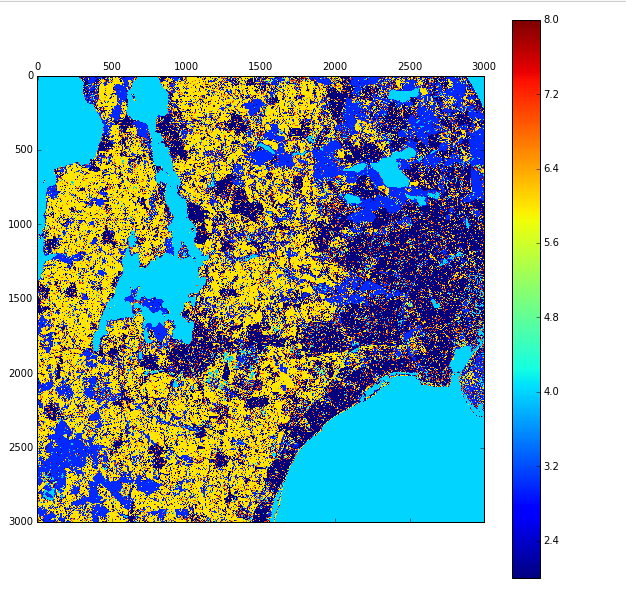
\includegraphics[width=10cm]{trees_pred.png}


\subsection{Runtime}
\subsection{Detecting Rare Instances}

\section{Hadoop}
\subsection{Airline Statistics}

\subsubsection*{a) Shortest Flight Distance}
\lstinputlisting[language={},numbers=left,numberstyle=\tiny,frame=single,breaklines=true,postbreak=\mbox{\textcolor{red}{$\hookrightarrow$}\space}]{../src/5_hadoop/1a_shortest_flight_distance/out/part-00000.}
\lstinputlisting[language={},numbers=left,numberstyle=\tiny,frame=single,breaklines=true,postbreak=\mbox{\textcolor{red}{$\hookrightarrow$}\space}]{../src/5_hadoop/1a_shortest_flight_distance/hrun.out}


\subsubsection*{b) Late Arrival Counts}
\lstinputlisting[language={},numbers=left,numberstyle=\tiny,frame=single,breaklines=true,postbreak=\mbox{\textcolor{red}{$\hookrightarrow$}\space}]{../src/5_hadoop/1b_late_arrival_counts/out/part-00000.}
\lstinputlisting[language={},numbers=left,numberstyle=\tiny,frame=single,breaklines=true,postbreak=\mbox{\textcolor{red}{$\hookrightarrow$}\space}]{../src/5_hadoop/1b_late_arrival_counts/hrun.out}


\subsubsection*{c) Mean and Standard deviation for Arrival Delay}
\lstinputlisting[language={},numbers=left,numberstyle=\tiny,frame=single,breaklines=true,postbreak=\mbox{\textcolor{red}{$\hookrightarrow$}\space}]{../src/5_hadoop/1c_mean_std_arrival_delay/out/part-00000.}
\lstinputlisting[language={},numbers=left,numberstyle=\tiny,frame=single,breaklines=true,postbreak=\mbox{\textcolor{red}{$\hookrightarrow$}\space}]{../src/5_hadoop/1c_mean_std_arrival_delay/hrun.out}

\subsubsection*{d) Top-10 Arrival Delays}
\lstinputlisting[language={},numbers=left,numberstyle=\tiny,frame=single,breaklines=true,postbreak=\mbox{\textcolor{red}{$\hookrightarrow$}\space}]{../src/5_hadoop/1d_top10_arrival_delays/out/part-00000.}
\lstinputlisting[language={},numbers=left,numberstyle=\tiny,frame=single,breaklines=true,postbreak=\mbox{\textcolor{red}{$\hookrightarrow$}\space}]{../src/5_hadoop/1d_top10_arrival_delays/hrun.out}


\subsection{Landsat Statistics}
\lstinputlisting[language={},numbers=left,numberstyle=\tiny,frame=single,breaklines=true,postbreak=\mbox{\textcolor{red}{$\hookrightarrow$}\space}]{../src/5_hadoop/2_landsat_stats/out/part-00000.}

\lstinputlisting[language={},numbers=left,numberstyle=\tiny,frame=single,breaklines=true,postbreak=\mbox{\textcolor{red}{$\hookrightarrow$}\space}]{../src/5_hadoop/2_landsat_stats/hrun.out}



\section*{Appendix} 

\begin{figure}[!h]
	\centering
	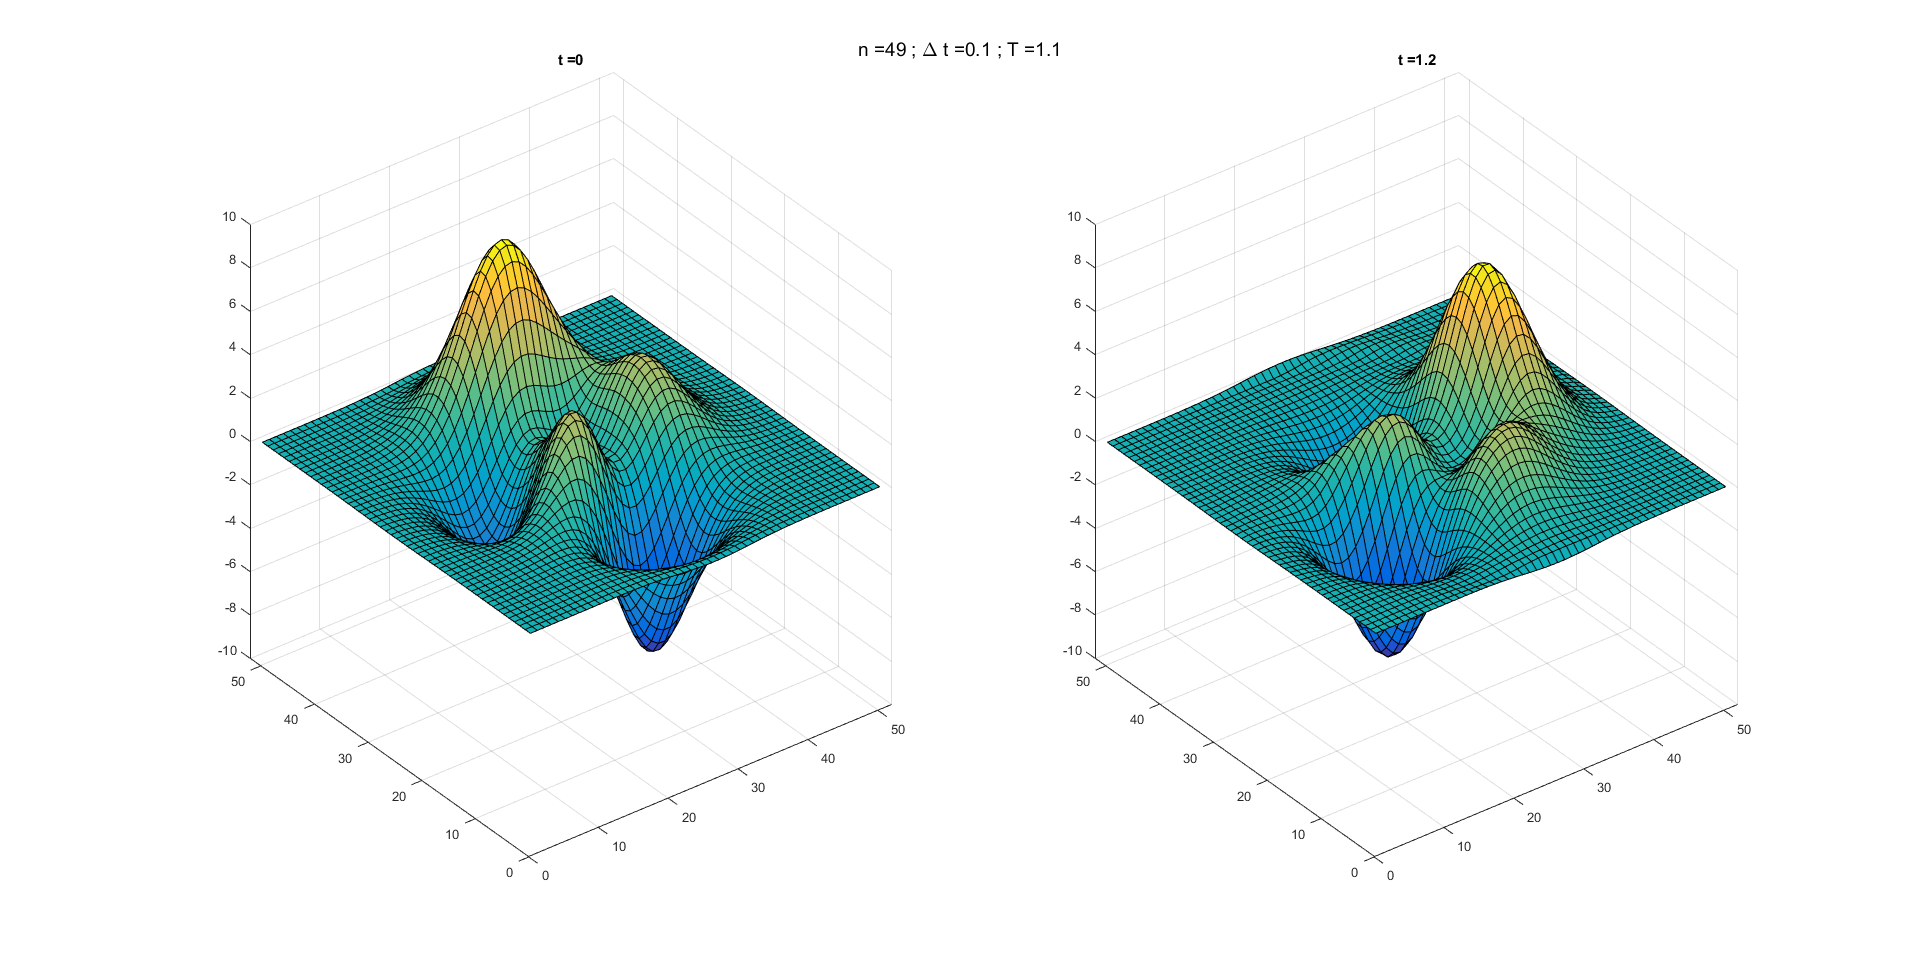
\includegraphics[width=160mm]{someplot}
\end{figure}


\printbibliography
\end{document}
